% Options for packages loaded elsewhere
\PassOptionsToPackage{unicode}{hyperref}
\PassOptionsToPackage{hyphens}{url}
%
\documentclass[
  10pt,
  ,
  french,
  a4paper]{article}
\usepackage{lmodern}
\usepackage{amsmath}
\usepackage{ifxetex,ifluatex}
\ifnum 0\ifxetex 1\fi\ifluatex 1\fi=0 % if pdftex
  \usepackage[T1]{fontenc}
  \usepackage[utf8]{inputenc}
  \usepackage{textcomp} % provide euro and other symbols
  \usepackage{amssymb}
\else % if luatex or xetex
  \usepackage{unicode-math}
  \defaultfontfeatures{Scale=MatchLowercase}
  \defaultfontfeatures[\rmfamily]{Ligatures=TeX,Scale=1}
\fi
% Use upquote if available, for straight quotes in verbatim environments
\IfFileExists{upquote.sty}{\usepackage{upquote}}{}
\IfFileExists{microtype.sty}{% use microtype if available
  \usepackage[]{microtype}
  \UseMicrotypeSet[protrusion]{basicmath} % disable protrusion for tt fonts
}{}
\makeatletter
\@ifundefined{KOMAClassName}{% if non-KOMA class
  \IfFileExists{parskip.sty}{%
    \usepackage{parskip}
  }{% else
    \setlength{\parindent}{0pt}
    \setlength{\parskip}{6pt plus 2pt minus 1pt}}
}{% if KOMA class
  \KOMAoptions{parskip=half}}
\makeatother
\usepackage{xcolor}
\IfFileExists{xurl.sty}{\usepackage{xurl}}{} % add URL line breaks if available
\IfFileExists{bookmark.sty}{\usepackage{bookmark}}{\usepackage{hyperref}}
\hypersetup{
  pdflang={french},
  hidelinks,
  pdfcreator={LaTeX via pandoc}}
\urlstyle{same} % disable monospaced font for URLs
\usepackage[margin=0.80in]{geometry}
\usepackage{color}
\usepackage{fancyvrb}
\newcommand{\VerbBar}{|}
\newcommand{\VERB}{\Verb[commandchars=\\\{\}]}
\DefineVerbatimEnvironment{Highlighting}{Verbatim}{commandchars=\\\{\}}
% Add ',fontsize=\small' for more characters per line
\usepackage{framed}
\definecolor{shadecolor}{RGB}{248,248,248}
\newenvironment{Shaded}{\begin{snugshade}}{\end{snugshade}}
\newcommand{\AlertTok}[1]{\textcolor[rgb]{0.94,0.16,0.16}{#1}}
\newcommand{\AnnotationTok}[1]{\textcolor[rgb]{0.56,0.35,0.01}{\textbf{\textit{#1}}}}
\newcommand{\AttributeTok}[1]{\textcolor[rgb]{0.77,0.63,0.00}{#1}}
\newcommand{\BaseNTok}[1]{\textcolor[rgb]{0.00,0.00,0.81}{#1}}
\newcommand{\BuiltInTok}[1]{#1}
\newcommand{\CharTok}[1]{\textcolor[rgb]{0.31,0.60,0.02}{#1}}
\newcommand{\CommentTok}[1]{\textcolor[rgb]{0.56,0.35,0.01}{\textit{#1}}}
\newcommand{\CommentVarTok}[1]{\textcolor[rgb]{0.56,0.35,0.01}{\textbf{\textit{#1}}}}
\newcommand{\ConstantTok}[1]{\textcolor[rgb]{0.00,0.00,0.00}{#1}}
\newcommand{\ControlFlowTok}[1]{\textcolor[rgb]{0.13,0.29,0.53}{\textbf{#1}}}
\newcommand{\DataTypeTok}[1]{\textcolor[rgb]{0.13,0.29,0.53}{#1}}
\newcommand{\DecValTok}[1]{\textcolor[rgb]{0.00,0.00,0.81}{#1}}
\newcommand{\DocumentationTok}[1]{\textcolor[rgb]{0.56,0.35,0.01}{\textbf{\textit{#1}}}}
\newcommand{\ErrorTok}[1]{\textcolor[rgb]{0.64,0.00,0.00}{\textbf{#1}}}
\newcommand{\ExtensionTok}[1]{#1}
\newcommand{\FloatTok}[1]{\textcolor[rgb]{0.00,0.00,0.81}{#1}}
\newcommand{\FunctionTok}[1]{\textcolor[rgb]{0.00,0.00,0.00}{#1}}
\newcommand{\ImportTok}[1]{#1}
\newcommand{\InformationTok}[1]{\textcolor[rgb]{0.56,0.35,0.01}{\textbf{\textit{#1}}}}
\newcommand{\KeywordTok}[1]{\textcolor[rgb]{0.13,0.29,0.53}{\textbf{#1}}}
\newcommand{\NormalTok}[1]{#1}
\newcommand{\OperatorTok}[1]{\textcolor[rgb]{0.81,0.36,0.00}{\textbf{#1}}}
\newcommand{\OtherTok}[1]{\textcolor[rgb]{0.56,0.35,0.01}{#1}}
\newcommand{\PreprocessorTok}[1]{\textcolor[rgb]{0.56,0.35,0.01}{\textit{#1}}}
\newcommand{\RegionMarkerTok}[1]{#1}
\newcommand{\SpecialCharTok}[1]{\textcolor[rgb]{0.00,0.00,0.00}{#1}}
\newcommand{\SpecialStringTok}[1]{\textcolor[rgb]{0.31,0.60,0.02}{#1}}
\newcommand{\StringTok}[1]{\textcolor[rgb]{0.31,0.60,0.02}{#1}}
\newcommand{\VariableTok}[1]{\textcolor[rgb]{0.00,0.00,0.00}{#1}}
\newcommand{\VerbatimStringTok}[1]{\textcolor[rgb]{0.31,0.60,0.02}{#1}}
\newcommand{\WarningTok}[1]{\textcolor[rgb]{0.56,0.35,0.01}{\textbf{\textit{#1}}}}
\usepackage{longtable,booktabs}
\usepackage{calc} % for calculating minipage widths
% Correct order of tables after \paragraph or \subparagraph
\usepackage{etoolbox}
\makeatletter
\patchcmd\longtable{\par}{\if@noskipsec\mbox{}\fi\par}{}{}
\makeatother
% Allow footnotes in longtable head/foot
\IfFileExists{footnotehyper.sty}{\usepackage{footnotehyper}}{\usepackage{footnote}}
\makesavenoteenv{longtable}
\usepackage{graphicx}
\makeatletter
\def\maxwidth{\ifdim\Gin@nat@width>\linewidth\linewidth\else\Gin@nat@width\fi}
\def\maxheight{\ifdim\Gin@nat@height>\textheight\textheight\else\Gin@nat@height\fi}
\makeatother
% Scale images if necessary, so that they will not overflow the page
% margins by default, and it is still possible to overwrite the defaults
% using explicit options in \includegraphics[width, height, ...]{}
\setkeys{Gin}{width=\maxwidth,height=\maxheight,keepaspectratio}
% Set default figure placement to htbp
\makeatletter
\def\fps@figure{htbp}
\makeatother
\setlength{\emergencystretch}{3em} % prevent overfull lines
\providecommand{\tightlist}{%
  \setlength{\itemsep}{0pt}\setlength{\parskip}{0pt}}
\setcounter{secnumdepth}{5}
\usepackage[T1]{fontenc}
\usepackage{caption}
\usepackage{graphicx}
\usepackage{natbib}
\usepackage{fontawesome5}
\usepackage{subcaption}
\usepackage{amsfonts}
\usepackage{dsfont}
\usepackage{bbold}
\usepackage{xspace}
\usepackage{enumitem}
\usepackage{pifont}
\usepackage{wrapfig}
\usepackage{textpos}
\usepackage{array}
\usepackage{multicol}
\ifxetex
  % Load polyglossia as late as possible: uses bidi with RTL langages (e.g. Hebrew, Arabic)
  \usepackage{polyglossia}
  \setmainlanguage[]{}
\else
  \usepackage[shorthands=off,main=]{babel}
\fi
\ifluatex
  \usepackage{selnolig}  % disable illegal ligatures
\fi

\title{~\includegraphics[width=\textwidth,height=2.5cm]{img/LOGO-ENSAE.png}\\
\hspace*{0.333em}\textsc{Applied macroeconometrics}\\
\hspace*{0.333em}Les effets d'une hausse de l'Euribor 3-mois}
\author{Valentin Giust, Gautier Lenfant et Alain Quartier-la-Tente}
\date{}

\begin{document}
\maketitle

{
\setcounter{tocdepth}{2}
\tableofcontents
}
\vfill

L'ensemble du projet est disponible à l'adresse \url{https://github.com/AQLT/AppliedMacroEuribor} (à eventuellement modifier).

\newpage

\hypertarget{introduction}{%
\section*{Introduction}\label{introduction}}
\addcontentsline{toc}{section}{Introduction}

\begin{Shaded}
\begin{Highlighting}[]
\NormalTok{matrix }\OtherTok{\textless{}{-}} \FunctionTok{readRDS}\NormalTok{(}\StringTok{"../data/data.RDS"}\NormalTok{)}
\NormalTok{matrix }\OtherTok{\textless{}{-}} \FunctionTok{na.omit}\NormalTok{(matrix)}

\CommentTok{\#Select AIC{-}suggested lag\#}

\NormalTok{lagselect }\OtherTok{\textless{}{-}}\FunctionTok{VARselect}\NormalTok{(matrix,}\AttributeTok{lag.max=}\DecValTok{12}\NormalTok{,}\AttributeTok{type=}\StringTok{"both"}\NormalTok{)}
\NormalTok{lagselect}\SpecialCharTok{$}\NormalTok{selection}
\end{Highlighting}
\end{Shaded}

\begin{verbatim}
## AIC(n)  HQ(n)  SC(n) FPE(n) 
##     12      2      1      2
\end{verbatim}

\begin{Shaded}
\begin{Highlighting}[]
\NormalTok{p\_retenu }\OtherTok{=} \DecValTok{2}
\NormalTok{model}\OtherTok{\textless{}{-}}\FunctionTok{VAR}\NormalTok{(matrix, }\AttributeTok{p=}\NormalTok{p\_retenu,}\AttributeTok{type =} \StringTok{"const"}\NormalTok{)}

\DocumentationTok{\#\#\#Forecast Error Impulse Response\#\#\#}

\CommentTok{\#response of Unemployment to EURIBOR\#}
\NormalTok{forimp }\OtherTok{\textless{}{-}} \FunctionTok{irf}\NormalTok{(model, }\AttributeTok{impulse =} \StringTok{"EURIBOR\_3M"}\NormalTok{,}
           \AttributeTok{response =} \FunctionTok{c}\NormalTok{(}\StringTok{"unemployment"}\NormalTok{,}\StringTok{"dlGDP"}\NormalTok{,}\StringTok{"inflation"}\NormalTok{,}\StringTok{"underinf"}\NormalTok{),}
           \AttributeTok{n.ahead =} \DecValTok{8}\NormalTok{, }\AttributeTok{ortho =} \ConstantTok{FALSE}\NormalTok{, }\AttributeTok{runs =} \DecValTok{1000}\NormalTok{)}
\FunctionTok{plot}\NormalTok{(forimp,}\AttributeTok{plot.type=}\StringTok{"multiple"}\NormalTok{,}
     \AttributeTok{mar.multi =} \FunctionTok{c}\NormalTok{(.}\DecValTok{5}\NormalTok{, }\DecValTok{4}\NormalTok{, .}\DecValTok{5}\NormalTok{, }\DecValTok{4}\NormalTok{))}
\end{Highlighting}
\end{Shaded}

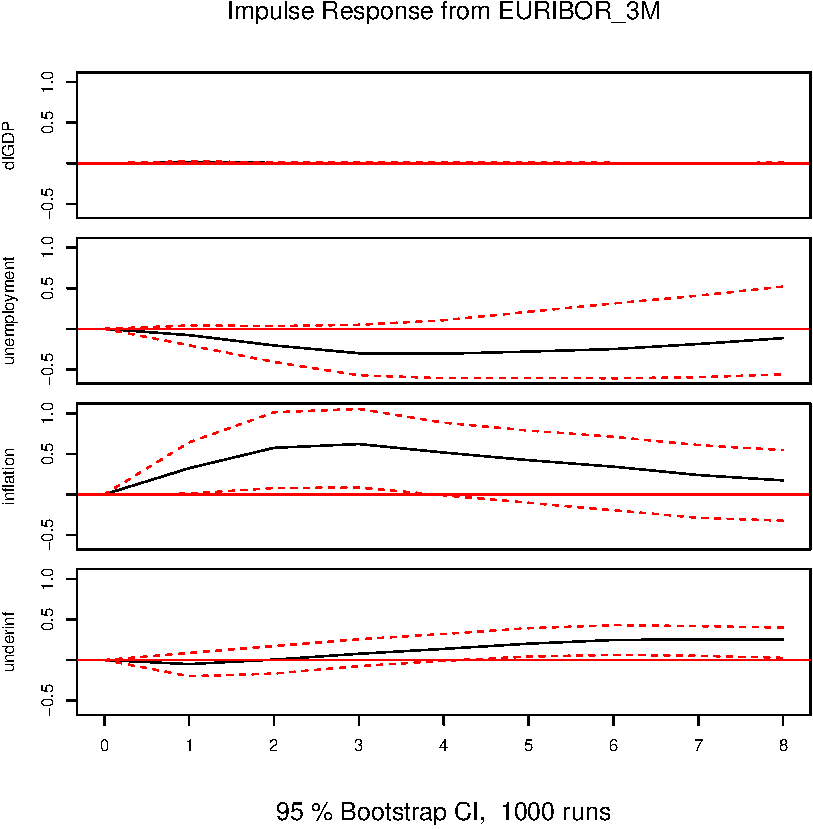
\includegraphics{img/markdown-unnamed-chunk-1-1.pdf}

\begin{Shaded}
\begin{Highlighting}[]
\DocumentationTok{\#\#\#Orthogonal Impulse Response\#\#\#}
\NormalTok{oir }\OtherTok{\textless{}{-}} \FunctionTok{irf}\NormalTok{(model, }\AttributeTok{impulse =} \StringTok{"EURIBOR\_3M"}\NormalTok{,}
           \AttributeTok{response =} \FunctionTok{c}\NormalTok{(}\StringTok{"unemployment"}\NormalTok{,}\StringTok{"dlGDP"}\NormalTok{,}\StringTok{"inflation"}\NormalTok{,}\StringTok{"underinf"}\NormalTok{),}
           \AttributeTok{n.ahead =} \DecValTok{8}\NormalTok{, }\AttributeTok{ortho =} \ConstantTok{TRUE}\NormalTok{, }\AttributeTok{runs =} \DecValTok{1000}\NormalTok{)}
\FunctionTok{plot}\NormalTok{(oir,}\AttributeTok{plot.type=}\StringTok{"multiple"}\NormalTok{,}
     \AttributeTok{mar.multi =} \FunctionTok{c}\NormalTok{(.}\DecValTok{5}\NormalTok{, }\DecValTok{4}\NormalTok{, .}\DecValTok{5}\NormalTok{, }\DecValTok{4}\NormalTok{))}
\end{Highlighting}
\end{Shaded}

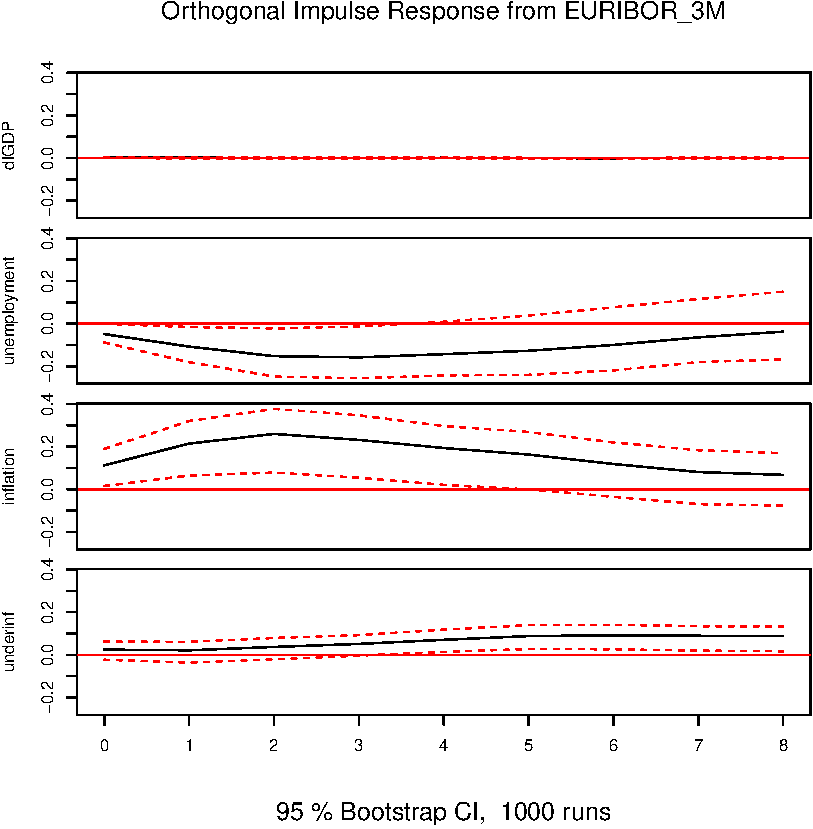
\includegraphics{img/markdown-unnamed-chunk-1-2.pdf}

\end{document}
